\chapter{Background and Literature Review}
\label{ch:review}

The goal of this chapter is to present the research context in which our project was conducted, by looking at common methods for each of the main components and highlighting those that inspired the current approach.

\section{Simultaneous Localization and Mapping (SLAM)}

SLAM constitutes a key research area in robotics, because it is a foundational building block for autonomous operation. This problem occurs when the robot does not have prior access to a map of the environment, so it must construct one while keeping track of its current position (\emph{online} SLAM). If the goal is to optimize the entire sequence of poses along the robot path, this is known as the \emph{full} SLAM problem. \cite{thrun}

Usually, the problem is discretized along the time dimension, such that at time $t$ we aim to compute the posterior function $p(x_t, M|z_{1:t}, u_{1:t})$, where $x_t$ is the current state, $M$ is the map, $z_{1:t}$ represents the set of measurements collected so far, and $u_{1:t}$ the control sequence. As each of these variables can have different concrete representations, depending on the task and the available sensors, a broad range of approaches have been proposed.

% KF and EKF
Aulinas et al. \cite{aulinas2008slam} note that the earliest methods rely on probabilistic models derived from the recursive Bayes rule, as such formulations can provide intuitive representations of the various noisy components involved in a robotic system. When employing the \acrfull{kf} \cite{Kalman1960} or its variations, the robot state, measurements and control inputs are modeled as multi-dimensional Gaussians, whose covariances describe the associated uncertainty. The algorithm alternates between \emph{predictions}, when the state is modified based on $u_t$, and \emph{updates}, when the prediction is evaluated against the latest observation $z_t$, and the state hypothesis is updated accordingly. The \acrfull{ekf} maintains this structure but can accommodate non-linearities in the displacement or measurement functions by using local linear approximations. Such methods have been successfully applied for indoor \cite{davisonEKF}, aerial \cite{luo2013uav}, and underwater \cite{palomer2019inspection} robots.

\acrfull{pf}, introduced by Del Moral \cite{del1997nonlinear}, is a probabilistic approach that relies on the Monte Carlo method. Instead of an analytical form, the uncertainty is accounted for by considering a large set of samples (representing potential states) and weighting them based on measurement likelihood. This has a higher computational cost than the standard KF methods, but is not affected by any linearization limitations. Nie et al. \cite{lcpf2020} implemented a LiDAR SLAM algorithm based on PF localization, albeit for 2D mapping.

Another large group of methods is represented by \emph{Visual SLAM}, when cameras are the main (and sometimes only) sensor used. As early as 1980, Moravec \cite{moravec1980obstacle} developed a robot capable of estimating its motion by matching features in images captured at discrete poses, in a stop-and-go fashion. In 2007, SLAM was being performed using a single handheld camera \cite{davison2007monoslam,klein2007parallel}, triggering a separation from the popular, offline, \gls{sfm} techniques. The solution is even more robust when a stereo system is available \cite{mei2011rslam}, as this helps avoid the geometrical limitations of monocular vision.

\section{Point cloud Registration}

Before discussing LiDAR-based approaches in more detail, let us review the task of point cloud registration. Given two sets of points $P, Q$ in arbitrary reference frames, representing (at least partially) the same scene, the goal is to find the transformation \mbox{$\matx{T} \in \SE{3}$} (translation and rotation) that best aligns the points. This can be expressed as an optimization problem:

\begin{equation}
    \underset{\matx{T}}{\operatorname{argmin}}\,J(\matx{T}P, Q)\comma
\end{equation}
where $J$ is a custom cost function. The particular case where known point correspondences are provided has a closed-form solution \cite{arun1987leastsquares}, but the \acrfull{icp} algorithm \cite{besl1992method} removes this constraint by alternating between correspondence generation --- each point in $P$ is paired with its nearest neighbor from $Q$ --- and minimizing the point-pair distances. This approach is by far the most widespread, thanks to its simplicity, computational efficiency (\eg using a \gls{kdtree} for closest-point search) and many available variations \cite{rusinkiewicz2001efficient,huang2021comprehensivesurveypointcloud}.

Chen and Medioni \cite{chen1991pointtoplane} proposed a ``point-to-plane'' minimization, while Segal et al. \cite{segal2009generalized} formulated a generalized cost function by considering the probabilistic model underlying the point sets, and implemented a ``plane-to-plane'' minimization. Other variants modify the point selection strategy \cite{masuda96icp,turk1994zippered}, apply a weight to each pair \cite{godin1994three}, prune the set of the correspondences \cite{pulli1999multiview,bouaziz2013sparse} or employ a different minimization algorithm \cite{blais1995registering}.

A different class of solutions operates by discretizing the space into \glspl{voxel} and estimating a normal distribution using the points in each voxel. Introduced in 2003, the \acrfull{ndt} \cite{biber2003normal} algorithm is the main competitor to ICP, enabling registration to be performed without the need for point-to-point correspondences. Magnusson et al. \cite{magnusson2007scan} extended this work to 3D scans, and performed a thorough comparison between this and ICP \cite{magnusson2009evaluation} for the challenging task of registering point clouds captured in underground mines, where few usable features are present. More recently, the method has been applied for outdoor mapping \cite{shen2024}, and as the basis for a Lidar Odometry and Mapping solution \cite{chen2021ndt}.

Neural Networks can also be used for point cloud registration, by creating correspondences based on features extracted by a descriptor architecture \cite{gojcic2019perfect,deng2018ppfnet}. This is particularly useful when no initial estimate of the transformation between the two point sets is available --- a scenario that the other approaches cannot directly handle.

\section{LiDAR-based Odometry and Mapping}

Despite their high price range, LiDAR sensors have gained significant popularity in the last decade, becoming the go-to solution for autonomous mobility. Unlike cameras, LiDARs are not dependent on ambient lighting, so they can operate in total darkness, and they provide high-frequency, reliable 3D information without the need for additional processing. Basic applications include obstacle detection \cite{asvadi20163d,chen2017lidar}, but the amount of information they provide makes them excellent for localization and mapping purposes.

\begin{figure}
    \centering
    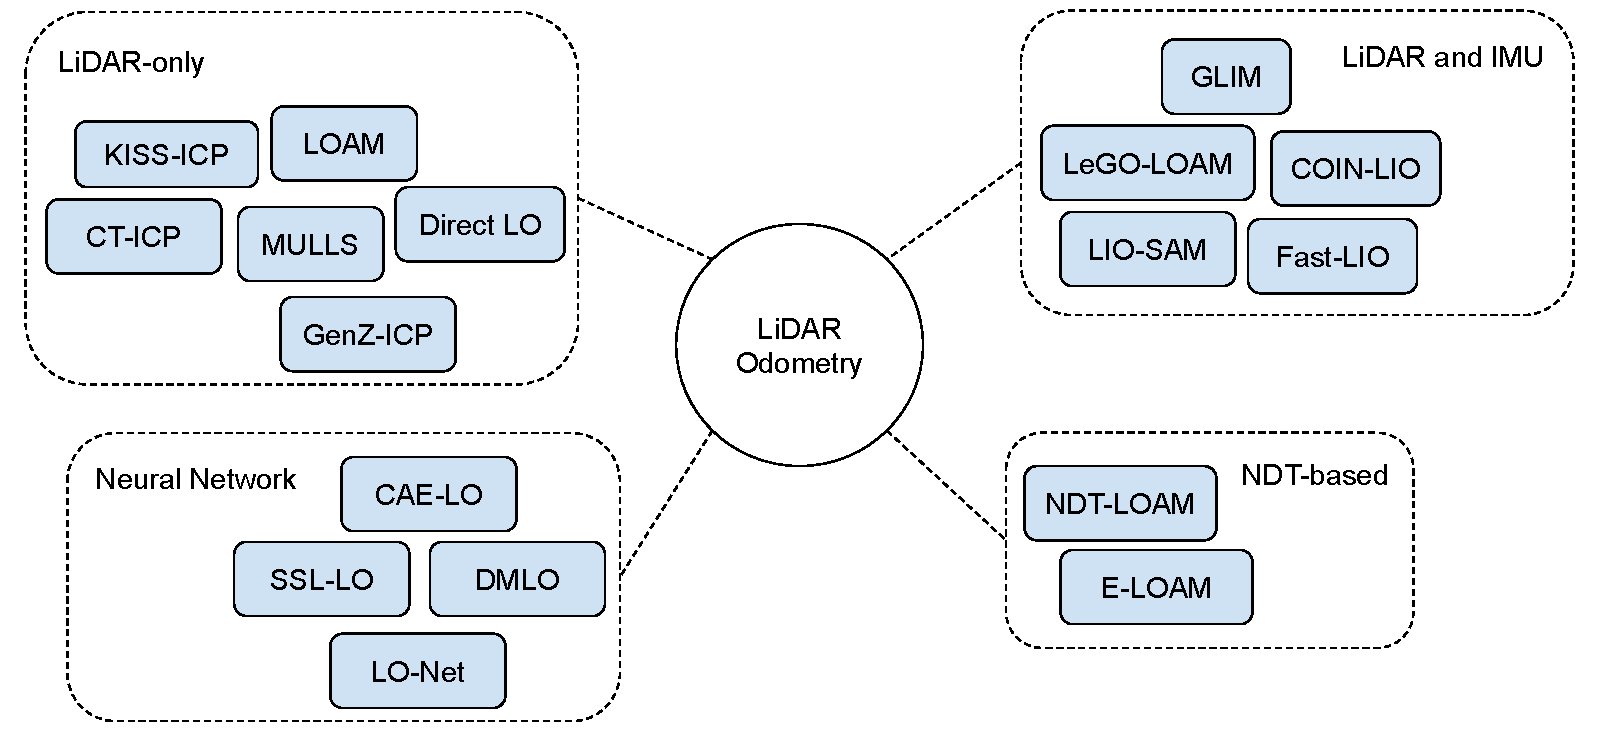
\includegraphics[width=0.6\linewidth]{images/lidar-odometry-tree.pdf}
    \caption[LiDAR Odometry Approaches]{A visualization of LiDAR odometry methods, grouped by approach: LOAM~\cite{zhang2014loam}, KISS-ICP~\cite{vizzo2023ral},  CT-ICP~\cite{dellenbach2021cticp}, MULLS~\cite{pan2021mulls}, Direct LO~\cite{chen2022directlo}, GenZ-ICP~\cite{lee2024genz}, GLIM~\cite{koide2024glim}, LeGO-LOAM~\cite{legoloam2018}, COIN-LIO~\cite{pfreundschuh2024coin}, LIO-SAM~\cite{shan2020lio}, Fast-LIO~\cite{fastlio}, CAE-LO~\cite{caelo2020}, SSL-LO~\cite{nubert2021self}, DMLO~\cite{li2020dmlo}, LO-Net~\cite{li2019net}, NDT-LOAM~\cite{chen2021ndt}, E-LOAM~\cite{guo2022loam}.}
    \label{fig:lidar-odometry-family}
\end{figure}


A key reference is \acrfull{loam}, the work of Zhang and Singh \cite{zhang2014loam}, who used a motorized, 2-axis LiDAR scanner to generate 3D point clouds. To register consecutive scans, they perform feature extraction (sharp edges or planar patches), identify correspondences to the previous scan, and find the optimal transformation using the Levenberg-Marquardt method \cite{levenberg1944method,marquardt}. To account for displacement during the beam sweep, points are reprojected by linear interpolation, assuming constant velocity --- this is known as \emph{motion/distortion compensation}. Mapping takes place in parallel, at a slower rate, and the current scan is registered to the map created so far. At that time, this implementation achieved the best results\footnote{\url{https://www.cvlibs.net/datasets/kitti/eval_odometry.php}} on the KITTI Odometry Benchmark \cite{geiger2012kitti}. V-LOAM \cite{zhang2015visual} improved this solution by introducing a visual odometry component based on a fish-eye camera.

A few years later, LeGO-LOAM \cite{legoloam2018} extended the feature extraction process by performing segmentation on a range image generated from the 3D point cloud. Clusters are filtered by size, in order to discard features belonging to potentially noisy points. Another modification is that the parameters of the transformation between consecutive scans are optimized separately: $t_z, \theta_{roll}, \theta_{pitch}$ are computed using planar feature correspondences, then fixed during the optimization of $t_x, t_y, \theta_{yaw}$, which only uses edge features. The method is compared to LOAM and achieves higher accuracy in outdoor scenarios, while being an order of magnitude faster.

F-LOAM \cite{wang2021f} proposes a two-step motion compensation process. For odometry computation, the constant velocity model is used, but the points are re-corrected using the optimized pose before being registered to the map. Correspondences are weighted based on the ``local smoothness'' of the feature, and the non-linear optimization is solved using the Gauss-Newton method. The map is not updated at every scan, but only when the translational change reaches a predefined threshold. This is a common \gls{keyframe} selection technique inherited from Visual Odometry.

A slightly different approach introduces the use of inertial sensors, leading to \acrfull{lio}. This aims to compensate for the lack of reliable 3D features in specific environments, as accelerometers can provide satisfactory motion estimates for short displacements. FAST-LIO \cite{fastlio} applies such a technique for a drone equipped with a high-frequency solid-state LiDAR, by performing tightly-coupled fusion: instead of using the IMU output to correct the scan registration, it is applied on the features extracted from the point cloud. COIN-LIO \cite{pfreundschuh2024coin} introduces a photometric error component, based on the beam intensity values returned by the LiDAR. A monochrome ``intensity image'' is constructed and filtered such that matching can occur between consecutive frames, and these new correspondences extend the residual vector that is minimized for odometry computation. The approach achieves state-of-the-art performance on a dataset of geometrically-degenerate scenes (ENWIDE \footnote{\url{https://projects.asl.ethz.ch/datasets/enwide}}).

% DMLO: Deep Matching LiDAR Odometry 2020 

In the class of deep-learning techniques, we highlight Deep Matching LiDAR Odometry (DMLO) \cite{li2020dmlo}, which translates the registration problem into a supervised machine learning task. Point clouds are projected into a 2D map using cylinder encoding, with range and intensity values as channels, and a \acrfull{cnn} architecture is trained to predict correspondences from pairs of projections. Training samples are constructed from a subset of the target dataset, and the method proves robust across different LiDAR hardware, but does not surpass LOAM on the KITTI sequences. In comparison to \cite{li2019net}, this solution does not leave the geometric problem to the inner workings of the CNN.

% KISS-ICP

The approach that our work draws most inspiration from is KISS-ICP \cite{vizzo2023ral}, a LiDAR-only odometry framework built around point-to-point ICP. This method proposes a few modifications that cooperate towards a hardware-agnostic solution, with a small number of adjustable parameters. The first contribution is a constant velocity motion estimation, which provides the optimization step with an initial guess. The same motion estimation is used for distortion compensation. Secondly, feature extraction is replaced by two stages of voxel-based down-sampling: the first down-sampled point cloud is used to extend the map, while the even lower-resolution set is registered against the existing map to compute the pose estimate. Perhaps the key component is an adaptive distance threshold for correspondence outlier removal. This threshold is updated based on the deviation between the predicted and optimized pose, acting as a form of uncertainty estimation. Additionally, the optimization problem employs a robust kernel, whose scale parameter is related to the adaptive threshold.

% ?
% \section{Industrial solutions}
